% !TEX root = ../../ctfp-reader.tex

\lettrine[lhang=0.17]{A}{ category is small} if its objects form a set. But we know that
there are things larger than sets. Famously, a set of all sets cannot be
formed within the standard set theory (the Zermelo-Fraenkel theory,
optionally augmented with the Axiom of Choice). So a category of all
sets must be large. There are mathematical tricks like Grothendieck
universes that can be used to define collections that go beyond sets.
These tricks let us talk about large categories.

A category is \emph{locally small} if morphisms between any two objects
form a set. If they don't form a set, we have to rethink a few
definitions. In particular, what does it mean to compose morphisms if we
can't even pick them from a set? The solution is to bootstrap ourselves
by replacing hom-sets, which are objects in $\Set$, with
\emph{objects} from some other category $\cat{V}$. The difference is
that, in general, objects don't have elements, so we are no longer
allowed to talk about individual morphisms. We have to define all
properties of an \emph{enriched} category in terms of operations that
can be performed on hom-objects as a whole. In order to do that, the
category that provides hom-objects must have additional structure --- it
must be a monoidal category. If we call this monoidal category $\cat{V}$,
we can talk about a category $\cat{C}$ enriched over $\cat{V}$.

Beside size reasons, we might be interested in generalizing hom-sets to
something that has more structure than mere sets. For instance, a
traditional category doesn't have the notion of a distance between
objects. Two objects are either connected by morphisms or not. All
objects that are connected to a given object are its neighbors. Unlike
in real life; in a category, a friend of a friend of a friend is as
close to me as my bosom buddy. In a suitably enriched category, we can
define distances between objects.

There is one more very practical reason to get some experience with
enriched categories, and that's because a very useful online source of
categorical knowledge, the \urlref{https://ncatlab.org/}{nLab}, is written
mostly in terms of enriched categories.

\section{Why Monoidal Category?}

When constructing an enriched category we have to keep in mind that we
should be able to recover the usual definitions when we replace the
monoidal category with $\Set$ and hom-objects with hom-sets. The
best way to accomplish this is to start with the usual definitions and
keep reformulating them in a point-free manner --- that is, without
naming elements of sets.

Let's start with the definition of composition. Normally, it takes a
pair of morphisms, one from $\cat{C}(b, c)$ and one from
$\cat{C}(a, b)$ and maps it to a morphism from $\cat{C}(a, c)$. In
other words it's a mapping:
\[\cat{C}(b, c)\times{}\cat{C}(a, b) \to \cat{C}(a, c)\]
This is a function between sets --- one of them being the Cartesian
product of two hom-sets. This formula can be easily generalized by
replacing Cartesian product with something more general. A categorical
product would work, but we can go even further and use a completely
general tensor product.

Next come the identity morphisms. Instead of picking individual elements
from hom-sets, we can define them using functions from the singleton set
$\cat{1}$:
\[j_a \Colon \cat{1} \to \cat{C}(a, a)\]
Again, we could replace the singleton set with the terminal object, but
we can go even further by replacing it with the unit $i$ of the
tensor product.

As you can see, objects taken from some monoidal category $\cat{V}$ are
good candidates for hom-set replacement.

\section{Monoidal Category}

We've talked about monoidal categories before, but it's worth restating
the definition. A monoidal category defines a tensor product that is a
bifunctor:
\[\otimes \Colon \cat{V}\times{}\cat{V} \to \cat{V}\]
We want the tensor product to be associative, but it's enough to satisfy
associativity up to natural isomorphism. This isomorphism is called the
associator. Its components are:
\[\alpha_{a\ b\ c} \Colon (a \otimes b) \otimes c \to a \otimes (b \otimes c)\]
It must be natural in all three arguments.

A monoidal category must also define a special unit object $i$
that serves as the unit of the tensor product; again, up to natural
isomorphism. The two isomorphisms are called, respectively, the left and
the right unitor, and their components are:
\begin{align*}
\lambda_a &\Colon i \otimes a \to a \\
\rho_a &\Colon a \otimes i \to a
\end{align*}
The associator and the unitors must satisfy coherence conditions:

\begin{figure}[H]
\centering
\begin{tikzcd}[row sep=large]
((a \otimes b) \otimes c) \otimes d
\arrow[d, "\alpha_{(a \otimes b)cd}"]
\arrow[rr, "\alpha_{abc} \otimes \id_d"]
  & & (a \otimes (b \otimes c)) \otimes d
      \arrow[d, "\alpha_{a(b \otimes c)d}"] \\
(a \otimes b) \otimes (c \otimes d)
\arrow[rd, "\alpha_{ab(c \otimes d)}"]
  & & a \otimes ((b \otimes c) \otimes d)
      \arrow[ld, "\id_a \otimes \alpha_{bcd}"] \\
  & a \otimes (b \otimes (c \otimes d))
\end{tikzcd}
\end{figure}

\begin{figure}[H]
\centering
\begin{tikzcd}[row sep=large]
(a \otimes i) \otimes b
\arrow[dr, "\rho_{a} \otimes \id_b"']
\arrow[rr, "\alpha_{aib}"]
  & & a \otimes (i \otimes b)
      \arrow[dl, "\id_a \otimes \lambda_b"] \\
  & a \otimes b
\end{tikzcd}
\end{figure}

\noindent
A monoidal category is called \newterm{symmetric} if there is a natural
isomorphism with components:
\[\gamma_{a\ b} \Colon a \otimes b \to b \otimes a\]
whose ``square is one'':
\[\gamma_{b\ a} \circ \gamma_{a\ b} = \idarrow[a \otimes b]\]
and which is consistent with the monoidal structure.

An interesting thing about monoidal categories is that you may be able
to define the internal hom (the function object) as the right adjoint to
the tensor product. You may recall that the standard definition of the
function object, or the exponential, was through the right adjoint to
the categorical product. A category in which such an object existed for
any pair of objects was called Cartesian closed. Here is the adjunction
that defines the internal hom in a monoidal category:
\[\cat{V}(a \otimes b, c) \sim \cat{V}(a, [b, c])\]
Following
\urlref{http://www.tac.mta.ca/tac/reprints/articles/10/tr10.pdf}{G. M.
Kelly}, I'm using the notation ${[}b, c{]}$ for the internal
hom. The counit of this adjunction is the natural transformation whose
components are called evaluation morphisms:
\[\varepsilon_{a\ b} \Colon ([a, b] \otimes a) \to b\]
Notice that, if the tensor product is not symmetric, we may define
another internal hom, denoted by ${[}{[}a, c{]}{]}$, using the
following adjunction:
\[\cat{V}(a \otimes b, c) \sim \cat{V}(b, [[a, c]])\]
A monoidal category in which both are defined is called \newterm{biclosed}. An
example of a category that is not biclosed is the category of
endofunctors in $\Set$, with functor composition serving as tensor
product. That's the category we used to define monads.

\section{Enriched Category}

A category $\cat{C}$ enriched over a monoidal category $\cat{V}$ replaces
hom-sets with hom-objects. To every pair of objects $a$ and
$b$ in $\cat{C}$ we associate an object $\cat{C}(a, b)$ in
$\cat{V}$. We use the same notation for hom-objects as we used for
hom-sets, with the understanding that they don't contain morphisms. On
the other hand, $\cat{V}$ is a regular (non-enriched) category with
hom-sets and morphisms. So we are not entirely rid of sets --- we just
swept them under the rug.

Since we cannot talk about individual morphisms in $\cat{C}$, composition
of morphisms is replaced by a family of morphisms in $\cat{V}$:
\[\circ \Colon \cat{C}(b, c) \otimes \cat{C}(a, b) \to \cat{C}(a, c)\]

\begin{figure}[H]
\centering
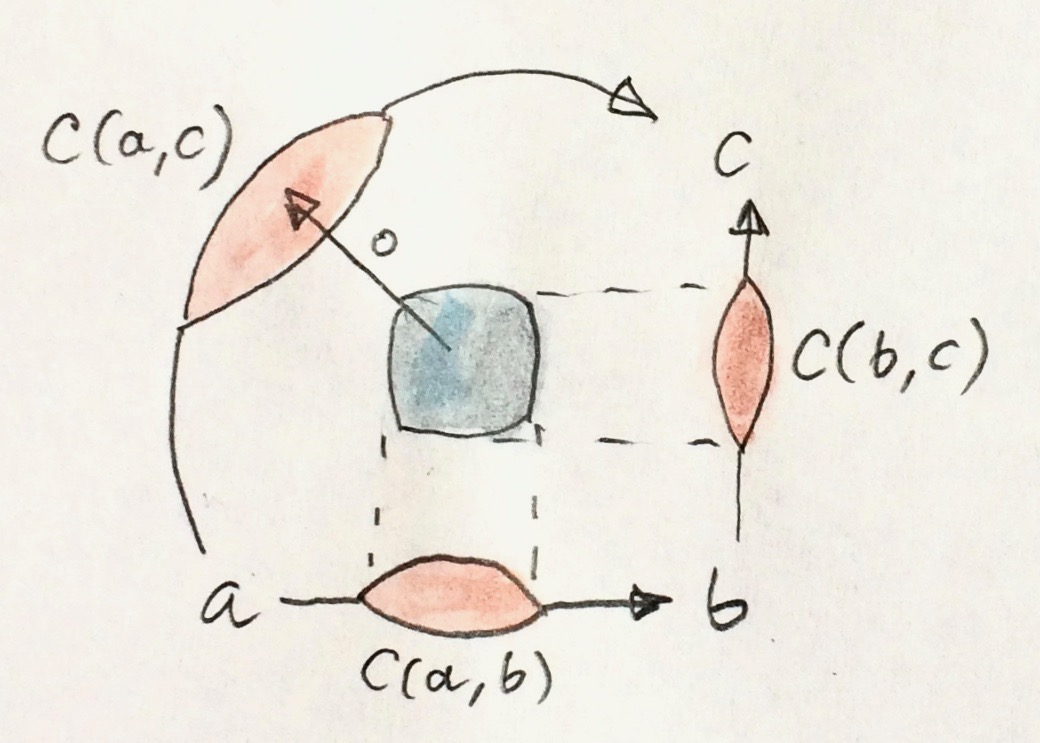
\includegraphics[width=60mm]{images/composition.jpg}
\end{figure}

\noindent
Similarly, identity morphisms are replaced by a family of morphisms in
$\cat{V}$:
\[j_a \Colon i \to \cat{C}(a, a)\]
where $i$ is the tensor unit in $\cat{V}$.

\begin{figure}[H]
\centering
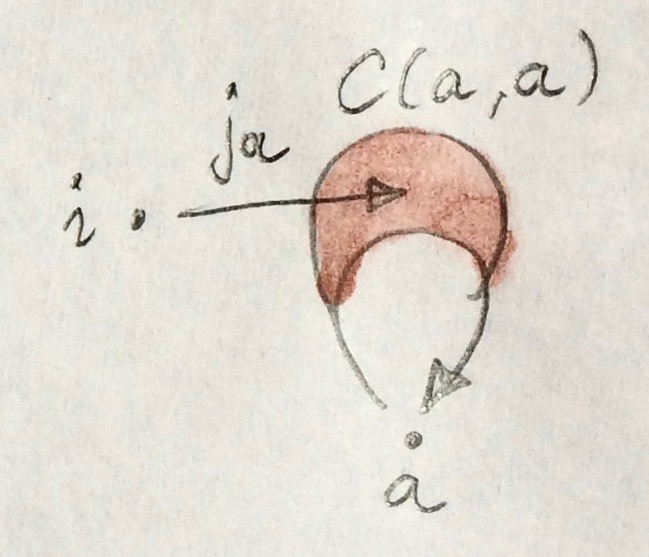
\includegraphics[width=40mm]{images/id.jpg}
\end{figure}

\noindent
Associativity of composition is defined in terms of the associator in
$\cat{V}$:

\begin{figure}[H]
\centering
\begin{tikzcd}[column sep=large]
(\cat{C}(c,d) \otimes \cat{C}(b,c)) \otimes \cat{C}(a,b)
\arrow[r, "\circ\otimes\id"]
\arrow[dd, "\alpha"]
  & \cat{C}(b,d) \otimes \cat{C}(a,b)
    \arrow[dr, "\circ"] \\
  & & \cat{C}(a,d) \\
\cat{C}(c,d) \otimes (\cat{C}(b,c) \otimes \cat{C}(a,b))
\arrow[r, "\id\otimes\circ"]
  & \cat{C}(c,d) \otimes \cat{C}(a,c)
    \arrow[ur, "\circ"]
\end{tikzcd}
\end{figure}

\noindent
Unit laws are likewise expressed in terms of unitors:

\begin{figure}[H]
  \centering
  \begin{subfigure}
    \centering
    \begin{tikzcd}[row sep=large]
      \cat{C}(a,b) \otimes i
      \arrow[rr, "\id \otimes j_a"]
      \arrow[dr, "\rho"]
        & & \cat{C}(a,b) \otimes \cat{C}(a,a)
            \arrow[dl, "\circ"] \\
        & \cat{C}(a,b)
    \end{tikzcd}
  \end{subfigure}
  \hspace{1cm}
  \begin{subfigure}
    \centering
    \begin{tikzcd}[row sep=large]
      i \otimes \cat{C}(a,b)
      \arrow[rr, "j_b \otimes \id"]
      \arrow[dr, "\lambda"]
        & & \cat{C}(b,b) \otimes \cat{C}(a,b)
            \arrow[dl, "\circ"] \\
        & \cat{C}(a,b)
    \end{tikzcd}
  \end{subfigure}
\end{figure}

\section{Preorders}

A preorder is defined as a thin category, one in which every hom-set is
either empty or a singleton. We interpret a non-empty set
$\cat{C}(a, b)$ as the proof that $a$ is less than or equal to
$b$. Such a category can be interpreted as enriched over a very
simple monoidal category that contains just two objects, $0$ and $1$
(sometimes called $False$ and $True$). Besides the mandatory identity
morphisms, this category has a single morphism going from $0$ to $1$, let's
call it $0 \to 1$. A simple monoidal structure can be
established in it, with the tensor product modeling the simple
arithmetic of $0$ and $1$ (i.e., the only non-zero product is $1 \otimes 1$).
The identity object in this category is $1$. This is a strict monoidal
category, that is, the associator and the unitors are identity
morphisms.

Since in a preorder the-hom set is either empty or a singleton, we can
easily replace it with a hom-object from our tiny category. The enriched
preorder $\cat{C}$ has a hom-object $\cat{C}(a, b)$ for any pair of
objects $a$ and $b$. If $a$ is less than or equal
to $b$, this object is $1$; otherwise it's $0$.

Let's have a look at composition. The tensor product of any two objects
is $0$, unless both of them are $1$, in which case it's $1$. If it's $0$, then
we have two options for the composition morphism: it could be either
$\idarrow[0]$ or $0 \to 1$. But if it's $1$, then the only
option is $\idarrow[1]$. Translating this back to relations, this says
that if $a \leqslant b$ and $b \leqslant c$ then
$a \leqslant c$, which is exactly the transitivity law we
need.

What about the identity? It's a morphism from $1$ to $\cat{C}(a, a)$.
There is only one morphism going from $1$, and that's the identity
$\idarrow[1]$, so $\cat{C}(a, a)$ must be $1$. It means that
$a \leqslant a$, which is the reflexivity law for a
preorder. So both transitivity and reflexivity are automatically
enforced, if we implement a preorder as an enriched category.

\section{Metric Spaces}

An interesting example is due to
\urlref{http://www.tac.mta.ca/tac/reprints/articles/1/tr1.pdf}{William
Lawvere}. He noticed that metric spaces can be defined using enriched
categories. A metric space defines a distance between any two objects.
This distance is a non-negative real number. It's convenient to include
infinity as a possible value. If the distance is infinite, there is no
way of getting from the starting object to the target object.

There are some obvious properties that have to be satisfied by
distances. One of them is that the distance from an object to itself
must be zero. The other is the triangle inequality: the direct distance
is no larger than the sum of distances with intermediate stops. We don't
require the distance to be symmetric, which might seem weird at first
but, as Lawvere explained, you can imagine that in one direction you're
walking uphill, while in the other you're going downhill. In any case,
symmetry may be imposed later as an additional constraint.

So how can a metric space be cast into a categorical language? We have
to construct a category in which hom-objects are distances. Mind you,
distances are not morphisms but hom-objects. How can a hom-object be a
number? Only if we can construct a monoidal category $\cat{V}$ in which
these numbers are objects. Non-negative real numbers (plus infinity)
form a total order, so they can be treated as a thin category. A
morphism between two such numbers $x$ and $y$ exists if
and only if $x \geqslant y$ (note: this is the opposite
direction to the one traditionally used in the definition of a
preorder). The monoidal structure is given by addition, with zero
serving as the unit object. In other words, the tensor product of two
numbers is their sum.

A metric space is a category enriched over such monoidal category. A
hom-object $\cat{C}(a, b)$ from object $a$ to $b$ is a
non-negative (possibly infinite) number that we will call the distance
from $a$ to $b$. Let's see what we get for identity and
composition in such a category.

By our definitions, a morphism from the tensorial unit, which is the
number zero, to a hom-object $\cat{C}(a, a)$ is the relation:
\[0 \geqslant \cat{C}(a, a)\]
Since $\cat{C}(a, a)$ is a non-negative number, this condition tells
us that the distance from $a$ to $a$ is always zero.
Check!

Now let's talk about composition. We start with the tensor product of
two abutting hom-objects, $\cat{C}(b, c) \otimes \cat{C}(a, b)$. We have defined
the tensor product as the sum of the two distances. Composition is a
morphism in $\cat{V}$ from this product to $\cat{C}(a, c)$. A morphism
in $\cat{V}$ is defined as the greater-or-equal relation. In other words,
the sum of distances from $a$ to $b$ and from $b$
to $c$ is greater than or equal to the distance from $a$
to $c$. But that's just the standard triangle inequality. Check!

By re-casting the metric space in terms of an enriched category, we get
the triangle inequality and the zero self-distance ``for free.''

\section{Enriched Functors}

The definition of a functor involves the mapping of morphisms. In the
enriched setting, we don't have the notion of individual morphisms, so
we have to deal with hom-objects in bulk. Hom-objects are objects in a
monoidal category $\cat{V}$, and we have morphisms between them at our
disposal. It therefore makes sense to define enriched functors between
categories when they are enriched over the same monoidal category
$\cat{V}$. We can then use morphisms in $\cat{V}$ to map the hom-objects
between two enriched categories.

An \newterm{enriched functor} $F$ between two categories $\cat{C}$
and $\cat{D}$, besides mapping objects to objects, also assigns, to every
pair of objects in $\cat{C}$, a morphism in $\cat{V}$:
\[F_{a\ b} \Colon \cat{C}(a, b) \to \cat{D}(F\ a, F\ b)\]
A functor is a structure-preserving mapping. For regular functors it
meant preserving composition and identity. In the enriched setting, the
preservation of composition means that the following diagram commute:

\begin{figure}[H]
\centering
\begin{tikzcd}[column sep=large, row sep=large]
  \cat{C}(b,c) \otimes \cat{C}(a,b)
  \arrow[r, "\circ"]
  \arrow[d, "F_{bc} \otimes F_{ab}"]
    & \cat{C}(a,c)
      \arrow[d, "F_{ac}"] \\
  \cat{D}(F\ b, F\ c) \otimes \cat{D}(F\ a, F\ b)
  \arrow[r,  "\circ"]
    & \cat{D}(F\ a, F\ c)
\end{tikzcd}
\end{figure}

\noindent
The preservation of identity is replaced by the preservation of the
morphisms in $\cat{V}$ that ``select'' the identity:

\begin{figure}[H]
\centering
\begin{tikzcd}[row sep=large]
    & i \arrow[dl, "j_a"'] \arrow[dr, "j_{F\ a}"] & \\
  \cat{C}(a,a)
  \arrow[rr, "F_{aa}"]
    & & \cat{D}(F\ a, F\ a)
\end{tikzcd}
\end{figure}

\section{Self Enrichment}

A closed symmetric monoidal category may be self-enriched by replacing
hom-sets with internal homs (see the definition above). To make this
work, we have to define the composition law for internal homs. In other
words, we have to implement a morphism with the following signature:
\[[b, c] \otimes [a, b] \to [a, c]\]
This is not much different from any other programming task, except that,
in category theory, we usually use point free implementations. We start
by specifying the set whose element it's supposed to be. In this case,
it's a member of the hom-set:
\[\cat{V}([b, c] \otimes [a, b], [a, c])\]
This hom-set is isomorphic to:
\[\cat{V}(([b, c] \otimes [a, b]) \otimes a, c)\]
I just used the adjunction that defined the internal hom
${[}a, c{]}$. If we can build a morphism in this new set, the
adjunction will point us at the morphism in the original set, which we
can then use as composition. We construct this morphism by composing
several morphisms that are at our disposal. To begin with, we can use
the associator $\alpha_{{[}b, c{]}\ {[}a, b{]}\ a}$ to reassociate the
expression on the left:
\[([b, c] \otimes [a, b]) \otimes a \to [b, c] \otimes ([a, b] \otimes a)\]
We can follow it with the co-unit of the adjunction $\varepsilon_{a\ b}$:
\[[b, c] \otimes ([a, b] \otimes a) \to [b, c] \otimes b\]
And use the counit $\varepsilon_{b\ c}$ again to get to $c$. We have
thus constructed a morphism:
\[\varepsilon_{b\ c}\ .\ (\idarrow[{[b, c]}] \otimes \varepsilon_{a\ b})\ .\ \alpha_{[b, c]\ [a, b]\ a}\]
that is an element of the hom-set:
\[\cat{V}(([b, c] \otimes [a, b]) \otimes a, c)\]
The adjunction will give us the composition law we were looking for.

Similarly, the identity:
\[j_a \Colon i \to [a, a]\]
is a member of the following hom-set:
\[\cat{V}(i, [a, a])\]
which is isomorphic, through adjunction, to:
\[\cat{V}(i \otimes a, a)\]
We know that this hom-set contains the left identity $\lambda_a$. We can
define $j_a$ as its image under the adjunction.

A practical example of self-enrichment is the category $\Set$ that
serves as the prototype for types in programming languages. We've seen
before that it's a closed monoidal category with respect to Cartesian
product. In $\Set$, the hom-set between any two sets is itself a
set, so it's an object in $\Set$. We know that it's isomorphic to
the exponential set, so the external and the internal homs are
equivalent. Now we also know that, through self-enrichment, we can use
the exponential set as the hom-object and express composition in terms
of Cartesian products of exponential objects.

\section{Relation to $\cat{2}$-Categories}

I talked about $\cat{2}$-categories in the context of $\Cat$, the category
of (small) categories. The morphisms between categories are functors,
but there is an additional structure: natural transformations between
functors. In a $\cat{2}$-category, the objects are often called zero-cells;
morphisms, $1$-cells; and morphisms between morphisms, $2$-cells. In
$\Cat$ the $0$-cells are categories, $1$-cells are functors, and
$2$-cells are natural transformations.

But notice that functors between two categories form a category too; so,
in $\Cat$, we really have a \emph{hom-category} rather than a
hom-set. It turns out that, just like $\Set$ can be treated as a
category enriched over $\Set$, $\Cat$ can be treated as a
category enriched over $\Cat$. Even more generally, just like
every category can be treated as enriched over $\Set$, every
$\cat{2}$-category can be considered enriched over $\Cat$.
